\documentclass[12pt,addpoints]{exam} 
\usepackage{amssymb, amsthm, amsmath, amscd, amsfonts}
\usepackage{graphicx}
\usepackage{verbatim}
\usepackage[all]{xy}
\usepackage{pgf,tikz}
\usepackage{xparse}
\usepackage{pythontex}

\newcommand{\RandomVoterGrid}[1]{%
  \pgfmathsetseed{#1}%
  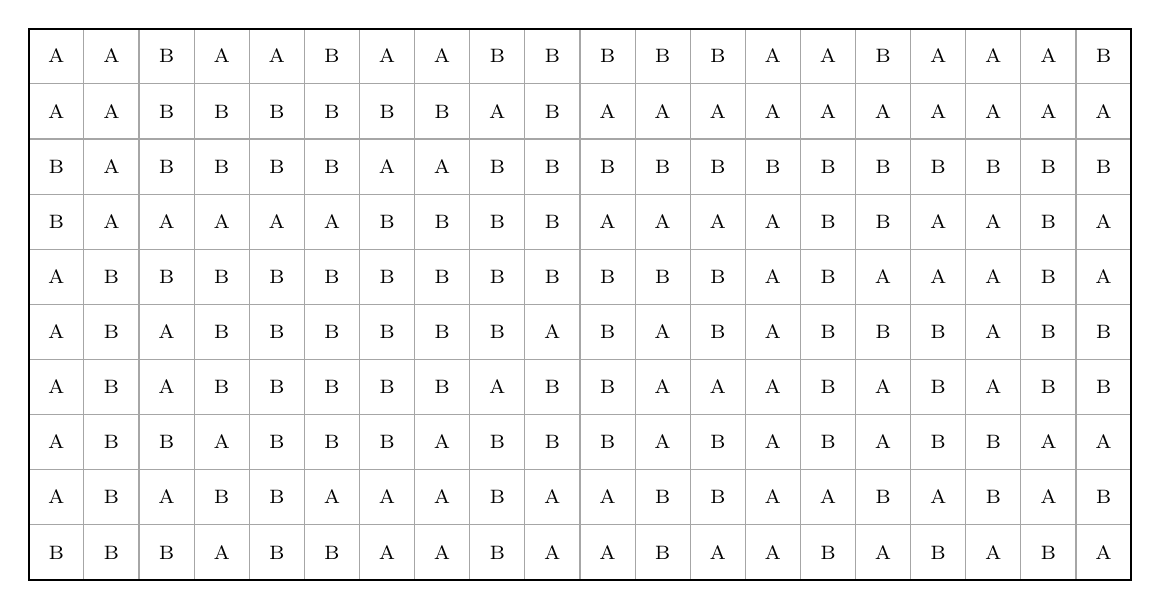
\begin{tikzpicture}[scale=0.7]
    \draw[step=1, gray!70, thin] (0,0) grid (20,10);
    \draw[black, thick] (0,0) rectangle (20,10);
    \foreach \x in {0,...,19} {
      \foreach \y in {0,...,9} {
        \pgfmathrandominteger{\r}{0}{1}
        \ifnum\r=0
          \node at (\x+0.5,\y+0.5) {\scriptsize A};
        \else
          \node at (\x+0.5,\y+0.5) {\scriptsize B};
        \fi
      }
    }
  \end{tikzpicture}%
}
\pagestyle{empty}

\begin{document}
\begin{center}
\RandomVoterGrid{1027} % seed: e.g. birthday MMDD, student ID, exam version, etc.

Seed: 1027
\end{center}

\clearpage

\begin{center}
\RandomVoterGrid{1134} % seed: e.g. birthday MMDD, student ID, exam version, etc.

Seed: 1134
\end{center}

\clearpage
\begin{center}
\RandomVoterGrid{413} % seed: e.g. birthday MMDD, student ID, exam version, etc.

Seed: 413
\end{center}

\clearpage
\begin{center}
\RandomVoterGrid{908} % seed: e.g. birthday MMDD, student ID, exam version, etc.

Seed: 908
\end{center}


\clearpage
\begin{center}
\RandomVoterGrid{1010} % seed: e.g. birthday MMDD, student ID, exam version, etc.

Seed: 1010
\end{center}


\clearpage
\begin{center}
\RandomVoterGrid{1122} % seed: e.g. birthday MMDD, student ID, exam version, etc.

Seed: 1122
\end{center}

\end{document}